\documentclass[fleqn]{article} % document instead of article?
\usepackage{kpfonts}
\usepackage[T1]{fontenc}
% \usepackage{ocgx2} %implements PDF Layers
\usepackage[colorlinks, urlcolor=blue, linkcolor=black]{hyperref}
\usepackage[inline]{enumitem}
\usepackage{tabularx}
\usepackage{amsmath}
\usepackage{amstext}
\usepackage{amsfonts}
\usepackage{ulem}
\usepackage[a4paper, total={498pt, 10in}]{geometry}
\usepackage{tabto}
\usepackage{graphicx}
\usepackage{textcomp}
\usepackage{gensymb}
\usepackage{wrapfig}
\usepackage{multicol}
% \usepackage{svg}
% \usepackage{multimedia}
\usepackage{esvect}
\usepackage[export]{adjustbox}
\usepackage{mathtools}  
\usepackage{amssymb}
\mathtoolsset{showonlyrefs}

\newenvironment{exercises}{\begin{enumerate*}[label=\alph*), itemjoin=\qquad]}{\end{enumerate*}}

\DeclareMathOperator{\tg}{tg}
\DeclareMathOperator{\ctg}{ctg}
\DeclareMathOperator{\arctg}{arctg}
\DeclareMathOperator{\arcctg}{arcctg}

\DeclareMathOperator{\jei}{\ jei\ }
\DeclareMathOperator{\ir}{\ ir\ }
\DeclareMathOperator{\arba}{\ arba\ }

\DeclareMathOperator{\half}{\frac{1}{2}}
\DeclareMathOperator{\third}{\frac{1}{3}}

\setlength{\parindent}{0pt}

\begin{document}
\renewcommand{\tablename}{Lentelė}
\renewcommand{\figurename}{Iliustracija}
\renewcommand{\vec}{\vv}
\pagestyle{plain}
\texttt{}
\hbadness=10001

\begin{center} {\Large Matematikos antrojo atsiskaitymo paruoštukas} \end{center}

\begin{center} \textbf{Vektoriai} \end{center}
\begin{multicols}{3}
    Skaliarinė sandauga ($\vec{a}\cdot\vec{b}$)

    $\vec{a}\cdot\vec{b} = \vec{a}.x\cdot\vec{b}.x  + \vec{a}.y\cdot\vec{b}.y$

    $\vec{a}\cdot\vec{b} = |\vec{a}|\cdot|\vec{b}|\cdot\cos\angle(\vec{a}, \vec{b})$ 

    Panašu į kampą tarp $a$ ir $b$.
    \vfill\null
    \columnbreak
    Vektorinė sandauga ($\vec{a}\times\vec{b}$)

    $\left(
    \begin{vmatrix} a_y & a_z \\ b_y & b_z \end{vmatrix},
    \begin{vmatrix} a_z & a_x \\ b_z & b_x \end{vmatrix},
    \begin{vmatrix} a_x & a_y \\ b_x & b_y \end{vmatrix}
    \right)$ 

    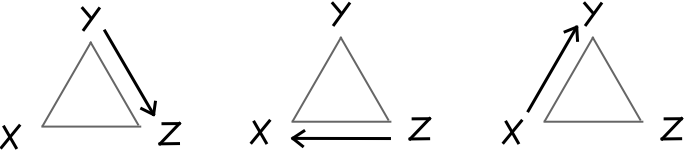
\includegraphics[scale=0.25]{assets/vektorine-daugyba.png}

    Duoda lygiagretainio plotą ir,

    padalinus iš 2, trikampio plotą

    \vfill\null
    \columnbreak
    Mišrioji sandauga ($(\vec{a}\vec{b}\vec{c})$)

    $(\vec{a}\times\vec{b})\cdot\vec{c} = \begin{vmatrix} a_x & a_y & a_z \\ b_x & b_y & b_z \\ c_x & c_y & c_z \end{vmatrix}$

    Duoda Prizmės tūrį ir 
    (padalinus iš 6)  
    trikampės piramidės turį.

\end{multicols}

\begin{center} \textbf{Plokštumos} \\ Bendra lygtis: $Ax + By + Cz + D = 0$ \end{center}
\begin{multicols}{4}
    $\vec{n}$ -- normalė \\
    $\vec{s}$ -- lygiagretus P \\
    \includegraphics[scale=0.25]{assets/plokštuma.png}
    \vfill\null
    \columnbreak

    Jei yra 3 taškai: \\
    $\vec{AM} = (x - 1; y - 2; z - 3)$ \\
    $\vec{AB} = (  4;     5;     6  )$ \\
    $\vec{AC} = (  7;     8;     9  )$ \\ 
    Po to skaičiuoti visų šitų skaičių determinantą
    \vfill\null
    \columnbreak

    Jei yra 2 taškai ir $\vec{s}$: \\
    $\vec{AM} = (x - 1; y - 2; z - 3)$ \\
    $\vec{AB} = (  4;     5;     6  )$ \\
    $\vec{s}  = (  7;     8;     9  )$ \\ 
    Po to skaičiuoti visų šitų skaičių determinantą
    \vfill\null
    \columnbreak

    Jei yra 2 taškai ir $\vec{n}$: \\
    $\vec{AM} = (x - 1; y - 2; z - 3)$ \\
    $\vec{n}  = (  4;     5;     6  )$ \\
    $4(x - 1) + 5(y - 2) + 6(z - 3)\nobreak=\nobreak 0$
\end{multicols}

\begin{center} \textbf{Tiesės} \end{center}
\begin{multicols}{2}
    Kanoninė lygtis: 
    $\frac{x - x_0}{l} = \frac{y - y_0}{m} = \frac{z - z_0}{n}$ \\
    Beje $(l; m; n)$ yra $\vec{s}$ (lygiagretus vektorius)
    \vfill\null
    \columnbreak

    Parametrinė lygtis:
    $\frac{x - x_0}{l} = \frac{y - y_0}{m} = \frac{z - z_0}{n} = t$ \\
    $\begin{cases} x = t + l\cdot x_0 \\ y = t + m\cdot y_0 \\ z = t + n\cdot z_0 \end{cases}$

\end{multicols}
\begin{multicols}{3}
    Kai taškas A ir $\vec{s}$: \\
    $A(...), M(x; y; z)$ \\
    $\vec{s}(...)$ \\ 
    $\frac{\vec{AM}_x}{\vec{s}_x} = ...$ \\
    \\
    Kai 2 taškai: \\
    $A(...), B(...)$ \\
    $M(x; y; z)$ \\
    $\frac{\vec{AM}_x}{\vec{AB}_x} = ...$

    \vfill\null
    \columnbreak

    Kai 2 plokštumos: \\
    $\begin{cases} 5x + 3y + 2z + 4 = 0\\ 2x + 8y - 9z - 10 = 0 \end{cases}$
    $M_0(x_0, y_0, 0)$ \\
    $\begin{cases} 5x_0 + 3y_0 + 2\cdot 0 + 4 = 0\\ 2x_0 + 8y_0 - 9\cdot 0 - 10 = 0 \end{cases}$ \\
    $\frac{x - x_0}{\begin{vmatrix} 3 & 2 \\ 8 & -9 \end{vmatrix}} = $
    $\frac{y - y_0}{\begin{vmatrix} 2 & 5 \\ -9 & 2 \end{vmatrix}} = \dots$

    \vfill\null
    \columnbreak

    Kampas tarp tiesės ir plokštumos: \\
    $\sin\varphi = \frac{\vec{s}\cdot\vec{n}}{|\vec{s}||\vec{n}|}$ \\
    Čia $\vec{n}$ koordinates reikia paiimti iš plokštumos lygties, \\
    o $\vec{s}$ yra tiesės kanoninės lygties apačioje(vardiklyje).

\end{multicols}

\begin{center} 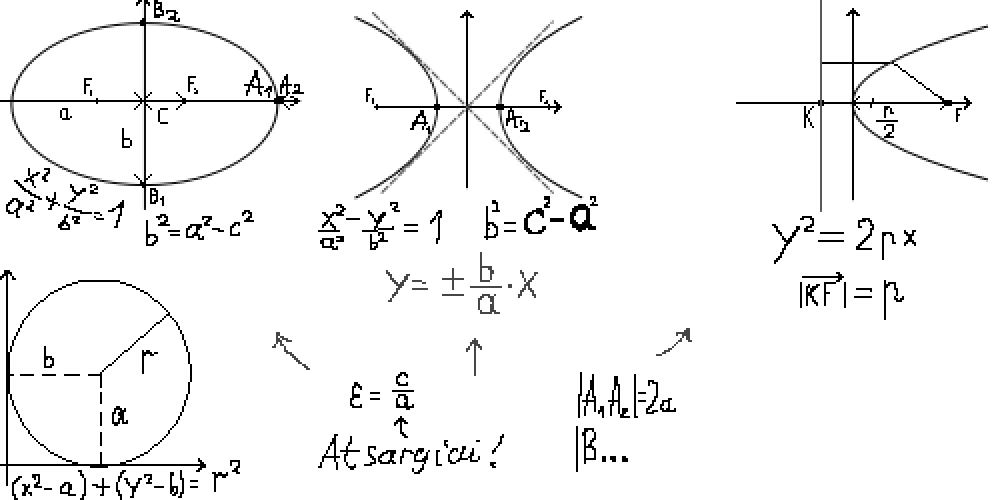
\includegraphics[scale=0.5]{assets/antros-eiles-kreives-2x.png} \end{center}

\pagenumbering{gobble}

\end{document}